\documentclass[conference]{IEEEtran}
\usepackage[utf8]{inputenc}
\usepackage{blindtext}
\usepackage{svg}
\usepackage{minted}
\usepackage{listings}
\definecolor{dkgreen}{rgb}{0,0.6,0}
\definecolor{ltgray}{rgb}{0.5,0.5,0.5}
\usepackage{todonotes}

\usepackage[hyphens]{url}
\usepackage{hyperref}
\hypersetup{breaklinks=true}
\usepackage{float}

\usepackage{listings}
\lstset{%
  	backgroundcolor=\color{white},
  	basicstyle=\footnotesize,
  	breakatwhitespace=false,
  	breaklines=true,
  	captionpos=b,
  	commentstyle=\color{dkgreen},
  	deletekeywords={...},
  	escapeinside={\%*}{*)},
  	extendedchars=true,
  	keepspaces=true,
  	keywordstyle=\color{blue},
  	language=SQL,
  	morekeywords={*,modify,MODIFY,...},
  	numbers=left,
  	numbersep=15pt,
  	numberstyle=\tiny,
  	rulecolor=\color{ltgray},
  	showspaces=false,
  	showstringspaces=false, 
  	showtabs=false,
  	stepnumber=1,
  	tabsize=4,
  	title=\lstname
}

\setminted{linenos, tabsize=2, fontsize=\footnotesize, xleftmargin=0.03\textwidth, breaklines}
\renewcommand{\listingautorefname{listing}}

\title{Command Query Responsibility Segregation in the field of spatial information}
\author{Jannes Neemann, Finn Beer and Darius Alter}

\date{April 2022}

\begin{document}

\maketitle

\begin{abstract}
Services that process or manage spatial data are subject to high scaling requirements, especially when the data has a global scope and is frequently modified. To meet these requirements, read operations can be separated from write operations. This approach is called Command Query Responsibility Segregation (CQRS), so that the read model can be scaled independently of the write model. The CQRS pattern is a good fit for spatial data and thus especially for map services such as OpenStreetMap (OSM).

Our implementation of the CQRS pattern shows that CQRS is well applicable to OSM. The Change Set Watcher component (CSW) generates individual events for each service that processes OSM data, including all state changes made to the write model of the OSM database. In this way, connected services can build their own read projection that contains only the data that the respective service needs.

The CSW was designed so that new services can be connected easily by subscribing to the individual events. As part of the implementation, a search service, a routing service and a render service were connected to the CSW. These services could all be scaled independently of each other and from the write model. State changes to the write model were made within a few seconds.
\end{abstract}

\begin{IEEEkeywords}
Command Query Responsibility Segregation, CQRS, Spatial Data, Event Processing, Vector Tiles, OpenStreetMap, OSM
\end{IEEEkeywords}

\section{Introduction}
\label{sec:Introduction}

Geospatial data used to be classically slow data. Data sets that were often managed and maintained by national agencies and government institutions were often published at intervals of several months. In today's world, where advanced technologies such as IOT devices with sensors are collecting data and linking it to geographic data, cartographic data is being created through crowdsourcing, and the overall speed at which data is being produced has accelerated. \cite{sveen_event-based_nodate} New methods are needed to process the data in a scalable way. In the following chapters, we will introduce the Command Query Responsibility Segregation Pattern (CQRS) and show its application and advantages in the context of spatial data.

We will start with an introduction to the design pattern and how it can be applied incrementally to an existing system. This is followed by a motivation why CQRS fits well with the data of OpenStreetMaps, which we refer to in particular in this paper. Afterwards, an introduction to the data types of OpenStreetMaps is given in order to understand our design decisions in our pipeline implementation.
To fulfill all elements of the pattern, we create a sample map application, which offers services for rendering, routing and searching. These exemplary services show how different applications with different data requirements can interact with the pipeline.


\section{CQRS}
\label{sec:cqrs}
In the course of domain-driven design, a domain model defines the structure of data, which provides the basis for storage in the database. It often happens that different clients update this data independently of each other and simultaneous. Clients usually do not process the data structures as intended by the original domain model or do not use the data in the same way.
Interaction with data is often done via CRUD APIs, which stand for Create, Read, Update, and Delete and do not separate the different activities such as reading and writing. Managing a single domain model that must manage all tasks to maintain consistency works well until clients need different views of the data. This is often the case when looking at microservice architectures.
Once a single domain model becomes too complex, there is an opportunity to use the Command Query Responsibility Segregation (CQRS) pattern to redesign the domain model to use separate operations for reading and writing. \cite{IBM_cqrs_2021}\\

CQRS separates write and query models, resulting in a simpler design and implementation of the system. The read models of the respective systems can be separately optimized for each underlying service and can be scaled without affecting its write data store \cite{noauthor_concepts_nodate}. Another advantage is that the development of the individual models can be carried out in parallel by different teams. It should be noted that the CQRS pattern results in a significant conceptual change to traditional patterns. Therefore, it should only be applied if the mentioned advantages are worth the effort. Using CQRS in an unsuitable environment leads to additional complexity, which can reduce productivity and increase risks. \cite{fowler_cqrs_2011}

The CQRS pattern consist of three different phases, which can be applied incrementally. 
Those phases determine how deeply the pattern should be applied to the existing architecture.
The first phase only contains a separation of the APIs. The second phase builds upon the first phase, but also contains a separation of the read and write domain models. However, these are still in a single database. Finally, in a full CQRS application, the databases are split into separate read and write databases. \cite{IBM_cqrs_2021}

When we consider a typical web application, the figure \ref{fig:cqrs_start} shows an application communicating with a single CRUD API to manage the underlying domain model, e.g., to edit, create, or read data. The first step in applying the CQRS pattern is to divide the APIs into separate read and write APIs. \cite{IBM_cqrs_2021} This step is called Command Query Separation (CQS) and describes the basic idea of dividing the methods of an object into two separate categories, queries and commands. The important part is that commands do not have a return value, but only return a status value like \textit{success}. The application of this step does not change the underlying data model, but only the access to the data. \cite{fowler_cqs_2005} However, this results in the disadvantage, that both are still highly coupled and thus can not be developed independently. 

\begin{figure}[h]
    \centering
    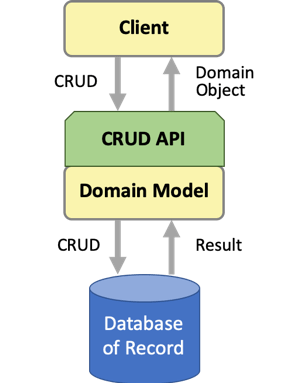
\includegraphics[width=0.2\textwidth]{figures/cqrs_start}
    \caption{Starting point - Typical Web-Application \cite{IBM_cqrs_2021}} 
    \label{fig:cqrs_start}
\end{figure}

The next step to achieve a deep integration of the pattern is the separation of the respective databases. However, the decoupling creates new complexity, as can be seen in figure \ref{fig:cqrs_full}. All changes that are made to the write model must also be passed on to the respective read models. This means that each change leads to the creation of an event, which is sent to the respective read databases by an event bus. Those events contain the changed information that the read model needs to create or to adjust its respective data. 


\begin{figure}[h]
    \centering
    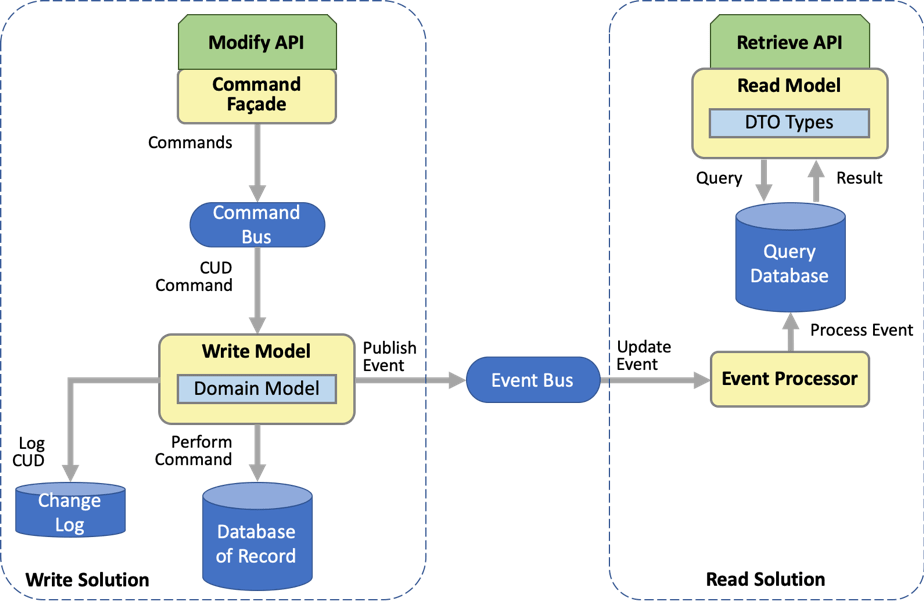
\includegraphics[width=0.45\textwidth]{figures/cqrs_full}
    \caption{CQRS - full pattern application \cite{IBM_cqrs_2021}}
    \label{fig:cqrs_full}
\end{figure}


\newpage


The second phase offers two decisive advantages: scaling and performance. the current load of requests can now be shifted from the write database to the read database. Furthermore, the read database can be replicated without considering the write database. In this case, it would only be necessary to send the change event to both read databases. The second advantage is performance. Since, in addition to the general separation of reading and writing, the schema has also been split. Both models can be designed and optimized independently of each other. The write database for example can be optimized for consistency and correctness and on the other hand the read database for application specific queries. This can result in e.g. larger rows with fewer joins, as well as completely new data structures. \cite{IBM_cqrs_2021}

It should be noted that the complexity is high, and it is a big risk to duplicate the data in two databases and keep them synchronized. Additionally, there is eventual consistency, since changes do not arrive directly in the read model after they have been made in the write model. \cite{noauthor_microservice_nodate}

\section{CQRS and OSM}
\label{sec:cqrs_osm}
Having introduced the CQRS pattern in the previous section, this section addresses why spatial data, and OSM data in particular, both require the CQRS pattern and why this kind of data fit CQRS.

Spatial data is information about objects, events or other features with a geographical reference \cite{ibm_gopspatialdata}. This can concern objects and events of the present as well as of the past (e.g. deconstructed roads). Spatial data with a global scope can grow large very quickly and can change very often. This results in large data streams and complex data structures. Services (e.g. map services) with such data have high scaling requirements. Map services such as OSM aim to map current and former transportation infrastructure, country boundaries, buildings, land uses, bodies of water, and point-of-interests worldwide. Thus, OSM data in particular requires a scalable infrastructure. Due to the property of OSM that many services using OSM only process or display the OSM data without modifying it, read and write operations may have different scaling requirements. Therefore, it is useful to separate the read model from the write model, which corresponds to the CQRS pattern. OSM already provides a write model. Write operations (commands) can be performed via the OSM editing API\footnote{OSM editing API: \url{https://api.openstreetmap.org/}}. Differing from the usual CQRS pattern, no classical events are sent via an event bus. All changes are described in \textit{OsmChange}-files at regular intervals. These change files contain the same information as the usual CQRS events. The main difference is that the read model itself must check if new change files are present. Whether the changes are published via an event bus or in change files, a sequence of state changes made to the write model is published. This concept is called event sourcing. \cite{maison_eventsourcing_2019}

Applying the CQRS pattern to OSM has the additional advantage that different services interested in different subsets of data can use their own read projections. To achieve this, the data must be preprocessed before it is stored in the read model. In the following sections, a component is presented that can perform this preprocessing for OSM data.

\section{OSM data structure}
For the remaining paper, it is important to understand the data structure of OpenStreetMap, which will be presented in the following section.

The OpenStreetMap database contains three types of so called \textit{OSM elements}: Nodes, Ways and Relations. With these elements all map structures (e.g. houses, streets, green areas etc.) can be mapped. All OSM elements contain a unique ID, an arbitrary number of tags, a version number, and a timestamp indicating the last time the element was edited. \cite{noauthor_elements_nodate} 

Nodes are the only elements that are directly associated with a geographic position. Thus, they contain both latitude and longitude coordinates. Since nodes are the only elements with geographic reference, they are referenced by other elements. 

Ways are the geometric representation of the geographical course of lines (e.g. roads, railroad lines, buildings, etc.). They contain an ordered list of node references. It is possible to decide between tree types of Ways \cite{osm_ways}: 
\begin{enumerate}
    \item \textbf{Open Ways}: Open ways begin and end at a different point. Thus, in an open way, the first and last node are not identical. Open ways can be used, for example, for roads or railroad lines.
    \item \textbf{Closed Ways}: If the last node is identical to the first node, the way is called closed. Closed ways can be used to model roundabouts and fences that enclose an area. 
    \item \textbf{Areas}: Areas are Closed Ways that either have an \texttt{area} tag or another tag that implies an area (e.g. \texttt{building})
\end{enumerate}
The third type of elements are relations. They are used to define logical or geographic relationships between different elements (e.g. train lines, turn restrictions, boundary lines, etc.). Relations contain a group of members which is an ordered list of one or more node, way and/or relation references. \cite{osm_relations}


Another important component of the OSM data structure are tags. Tags are used to represent properties, features and semantics of the elements just described \cite{osm_tags}. For example, a way, which in itself has no semantics and therefore is not shown on OSM maps, can become a road with the help of the \texttt{highway} tag (see \autoref{list:way_example}). The value of the tag specifies the described feature (e.g. the type of road). 

\begin{listing}[h]
    \inputminted{xml}{listings/way.xml}
    \caption{XML representation of a \texttt{way} element}
    \label{list:way_example}
\end{listing}
\section{Implementation}
\label{sec:Implementation}

\subsection{Architecture}
\label{subsec:Architecture}
\begin{figure*}[h]
  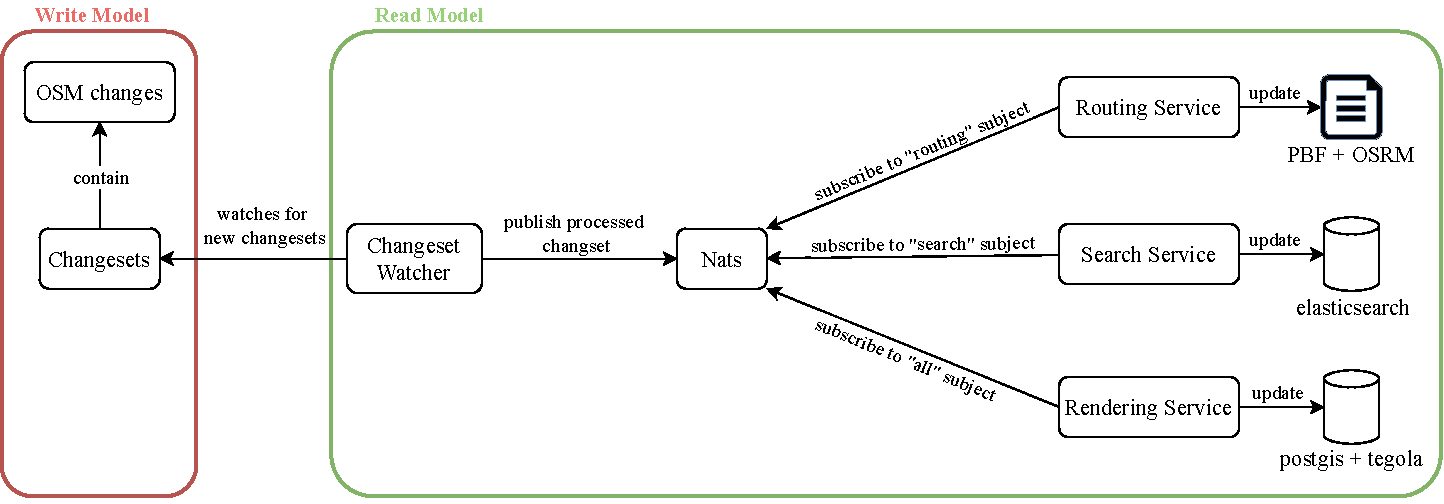
\includegraphics[height=6cm]{figures/architecture.pdf}
  \centering
  \caption{Pipeline Architecture}
  \label{fig:architecture}
\end{figure*}
As mentioned in section \ref{sec:cqrs_osm}, with larger data streams and higher data complexity, new methods are required to achieve a maintainable state. In order to apply the CQRS pattern to spatial data, we decided to build our own pipeline architecture as a proof of concept to show how the pattern can be applied.
As already described in section \ref{sec:cqrs}, the CQRS pattern consists in separating the write operations (commands) from the read operations (queries). This means that there is one database responsible for writing. While the reading part, also called projection, is derived from the writing part and can be managed by one or more databases. The reading part is asynchronous, which means that both parts are not strictly consistent. Since we are building our pipeline on top of changesets from OpenStreetMaps, we have to work with event sourced data. This means that we do not have a normal write database that distributes its changes trough events, but that the write model itself is a collection of events. This means that in the context of the pipeline presented here, the write model is not considered further, instead we will focus on the read model and how changes to the data are distributed asynchronously across the different projections. 

As can be seen in figure \ref{fig:architecture}, the entry point into the reading model is the Changeset-Watcher (CSW). The CSW performs a number of preprocessing and filtering operations, which are explained in more detail in section \ref{subsec:ChangesetWatcher}. After the preprocessing, it sends events to specific topics that can then be subscribed to by respective services (event processors) on the event bus. These services then receive these events and integrate the data into their own application-specific data models. We have decided to include three different services, each requiring a different data representation. 
One component handles searching, another routing and the last serving vector tiles for rendering. Together these service form a simple map application.
How the respective modules are structured and how they process the data arriving using events is described in more detail in the following sections. In our implementation, each module is build using Docker. The communication between containers therefore takes place over an internal Docker network, only targeted endpoints that need to be accessible via the frontend are accessible to the outside. Since the system is based on several modules, the use of containers facilitates the management of the individual modules.


\subsection{Changeset watcher}
The core of the implementation is the Changeset-Watcher (CSW). As soon as there is a state change at the write model and a new change file (OsmChange file) is available, it is downloaded by the CSW, preprocessed and distributed to all connected services in the desired form. The change files are provided via a NATS server. NATS \cite{noauthor_natsio_nodate}\cite{noauthor_natsdoc_nodate} is a lightweight message oriented middleware and allows any other services to be easily connected to the CSW. The CSW acts as a NATS client and publishes the preprocessed change files to specific subjects. A connected service subscribes to all subjects it needs for its purposes. The processing of the CSW can be divided into two sections: \textit{general preprocessing} and \textit{specific preprocessing} (see \autoref{fig:process_changeset_wa}).
\label{subsec:ChangesetWatcher}
\begin{figure}[h]
    \centering
    \includesvg[width=0.45\textwidth]{figures/process-changeset-wa.drawio.svg}
    \caption{Process of changeset watcher}
    \label{fig:process_changeset_wa}
\end{figure}
\subsubsection{Fetching and general preprocessing}
\label{sec:preprocessing}
The main data source of the CSW is the \textit{planet.osm} server. It makes both the current OpenStreetMap dataset and dataset changes publicly available. The OsmChange files summarize the minutely, hourly and daily changes. In these files, the nodes, ways or relations that have been changed in the minute, hour or day before are described. In order to provide the connected services with a state of the OpenStreetMap database that is as up-to-date as possible, only the OsmChange files with the minute-by-minute changes are considered\footnote{Minute-by-minute changes can be found under: \url{https://planet.openstreetmap.org/replication/minute/}}. In regular intervals (default is 10 seconds) the CSW checks if there is a new OsmChange file on the planet.osm server and downloads it if a new file has been detected.

Immediately after downloading, the change file is in a raw state, which is not optimal for further processing of the connected services:
\begin{itemize}
    \item \textbf{Complex Structure:} In the raw change file, changes from different users are listed in different modify, create and delete blocks. This increases the complexity of the data structure, although this subdivision does not provide any added value for further processing of the connected services.
    \item \textbf{Missing Nodes:} If way elements are changed (e.g. by adding tags), but the nodes that make up the way are not changed, the nodes are referenced by the way, but are not themselves listed in the change file (see lines 11-14 of \autoref{listing_raw_osc}). Without nodes, neither the connected services nor the CSW itself can determine the geographical location of the ways. 
    \item \textbf{Duplicate Elements:} If the same elements are changed several times within one minute, different versions of the elements appear in the change file (see lines 4 and 19 in \autoref{listing_raw_osc}).
\end{itemize}
In order to optimize the change files for subsequent further processing, they are preprocessed by the CSW. In the first step (see \autoref{fig:process_changeset_wa}), change files are normalized. I.e. the structure is simplified under changes of different users are listed in each case in a common modify, delete, or create block. In the second step, missing nodes are reloaded to enable the determination of the geographic location of the way. To do this, a POST-request is made to the overpass-API\footnote{Endpoint under \url{https://overpass-api.de/api/interpreter}} with all missing nodes. The response contains the corresponding nodes with the geographical positions. In the last step of the general preprocessing, all duplicates of elements are identified and removed. Only the newest element is kept.
\begin{listing}[h]
    \inputminted{xml}{listings/osmchange_raw.osc}
    \caption{Raw OsmChange file (simplified)}
    \label{listing_raw_osc}
\end{listing}

\subsubsection{Specific preprocessing}
The goal of our implementation is to ensure that each connected and reading service receives only the data it needs for its purpose. To achieve this goal, the change files must undergo a subject-specific preprocessing. In this process, the data is converted into exactly the form that the connected services require for further processing. These services can determine which OSM elements should be included, as well as in which format the files should be provided. To avoid the need to rewrite the source code of the specific preprocessing when a new service with new filter and format requirements is connected, or an existing service changes its requirements, we decided to outsource the filtering and format requirements to a simple configuration file. This even makes it possible to add new subjects or to change filters and output formats of existing subjects on the fly. In the configuration file, six different properties can be set for a subject (see \autoref{list:routing-configuration}):
\begin{itemize}
    \item \textbf{\texttt{Name}}: The value of this property specifies the name of the subject
    \item \textbf{\texttt{NodeFilters}}: This property can be used to select nodes to be published in the subject. The Value of this property is any number of \texttt{TagKeys} objects. For the filter condition to be matched, at least one \texttt{TagKeys} object must be true. For a \texttt{TagKeys} object to be true, the node must contain all tags of the \texttt{TagKeys} object. This allows both \texttt{AND} and \texttt{OR} relationships to be mapped. The null value means that the nodes should not be filtered and all nodes that are contained in the change file should be published.
    \item \textbf{\texttt{WayFilters}}: The functionality is the same as \texttt{NodeFilters} for ways instead of nodes. However, all nodes that are members of the ways that match the filter criteria will also pass. This is the case even if these nodes do not match the actual \texttt{NodeFilters}.
    \item \textbf{\texttt{Compress}}: Unfiltered change files in particular generate data volumes of several megabytes. To reduce the load on the event distribution and network, the change files can be compressed before the event is published.
    \item \textbf{\texttt{ReduceToPoints}}: For some applications, the exact type of OSM element is not relevant. In this case, the CSW offers to reduce nodes and ways (and thus also areas) to simple points. Points are defined by a geographic position and a name derived from the tags. In addition, the points contains all tags that the element had before the reduction. In the case of ways or areas, the geographic position is set to its centroid.
    \item \textbf{\texttt{Format}}: This CSW component offers \texttt{JSON} and \texttt{XML} as output formats. The last one is fully compatible with the OsmChange format.
\end{itemize}
\begin{listing}[h]
    \inputminted{json}{listings/config-routing.json}
    \caption{Configuration of subject \texttt{routing}}
    \label{list:routing-configuration}
\end{listing}
As shown in figure \ref{fig:process_changeset_wa}, different processing steps are triggered depending on the exact configuration for the subject. In this way, each connected service can build exactly the read projection it needs for further processing. In our implementation, three different services were connected to the CSW as an example, and a separate subject was configured for each of them. 

\subsection{Search}
\label{subsec:Search}
The search service is one of three representation of an exemplary read model. Its task is to quickly find the longitude and latitude of houses and points of interest through its associated tags (e.g. the house address). This service shall show how an arbitrary software module can be connected to our pipeline.
In our case, the search functionality is build using Elasticsearch \cite{noauthor_elasticsearch_nodate}, a robust search and analytic engine that supports full-text, fuzzy, and geospatial queries, as well as rapid indexing of frequently changing data. Elasticsearch uses a technique called inverted indexes as a data structure to find the respective items. Assuming our data to be indexed consists of a sentence for each data item. In order to quickly find those sentences, each sentence is split into its words. Every word is a key in the inverted index referencing the sentence in which it occurred. Therefore, sentences can be quickly found by just providing one word which is contained in the sentence. \cite{noauthor_elasticsearch_2013}
For this particular application, we decided to store only houses and amenities in a search point representation (see listing \ref{listing:searchpoint}) to keep the general model simple. 

\begin{listing}[h]
    \inputminted{json}{listings/searchpoint.json}
    \caption{Example Searchpoint}
    \label{listing:searchpoint}
\end{listing}

To transform the existing OSM data structures to search points, ways are aggregated to a single node with a recalculated centroid as the position. 
Therefore, ways that have the position stored as a polygon over multiple nodes can be treated the same as single nodes. This step is performed in the Changeset-Watcher within the specific subject filtering as shown in figure \ref{fig:process_changeset_wa}. 

To connect the service to the event bus, we need to configure which nodes and ways should be considered for the transformation through the dynamic filter configuration. In addition, we need to specify the name of the event that will be used to send this payload (see listing \ref{listing:searchConfig}). 

\begin{listing}[h]
    \inputminted{json}{listings/searchConfig.json}
    \caption{Search Filter Configuration}
    \label{listing:searchConfig}
\end{listing}

Elasticsearch itself has a REST-API that can be used to search or add new data to the store. Since we needed a small backend to handle event processing, we also added our own small REST-API, that abstracted the Elasticsearch API for easier access on the frontend.

\subsection{Rendering}
\label{subsec:Rendering}
The rendering service is the most important one when implementing a map application. Users orientate on the visual representation of geographic locations. Therefore, a rendering service translate geographic information into a visual form, mostly image based. In this specific case, the service must be capable of rendering OpenStreetMap data in the web. As the whole world has a lot of geographic information, it is not feasible to render one big image of the entire world, which is then served to the user over a web server. This image would have a resolution of multiple thousand gigapixel and hundreds of Gigabyte in size. Therefore, over the last years, the concept of a "tiled web map service" has become the de facto standard for serving map data in the web. All major map services e.g. Google Maps use this kind of concept. Fundamentally, a tiled web map service uses an \textit{image pyramid} in combination with image tiling, known as an \textit{image tile pyramid}. \cite{garcia12} Image pyramids were already known back in 1982 for creating multiresolution images \cite{in_e_1984}. Image tiles pyramids are also often used in the field of medicine, as they allow doctors to easily review digital tissue scans of multiple gigapixel, while preserving all the details needed for diagnosis \cite{Neemann2021}.
Figure \ref{fig:tile_pyramid} shows a representation of such a pyramid. It consists of multiple layers. The closer to the top, the coarser the resolution of the image. Closer to the base of the pyramid, the images are more detailed with higher resolution. Due to the image tiling, clients do not have to load the whole layer, but just those tiles that are actually visible in the browser. Therefore, improving performance. \cite{garcia12}\cite{netek_performance_2020}
\begin{figure}[h]
    \centering
    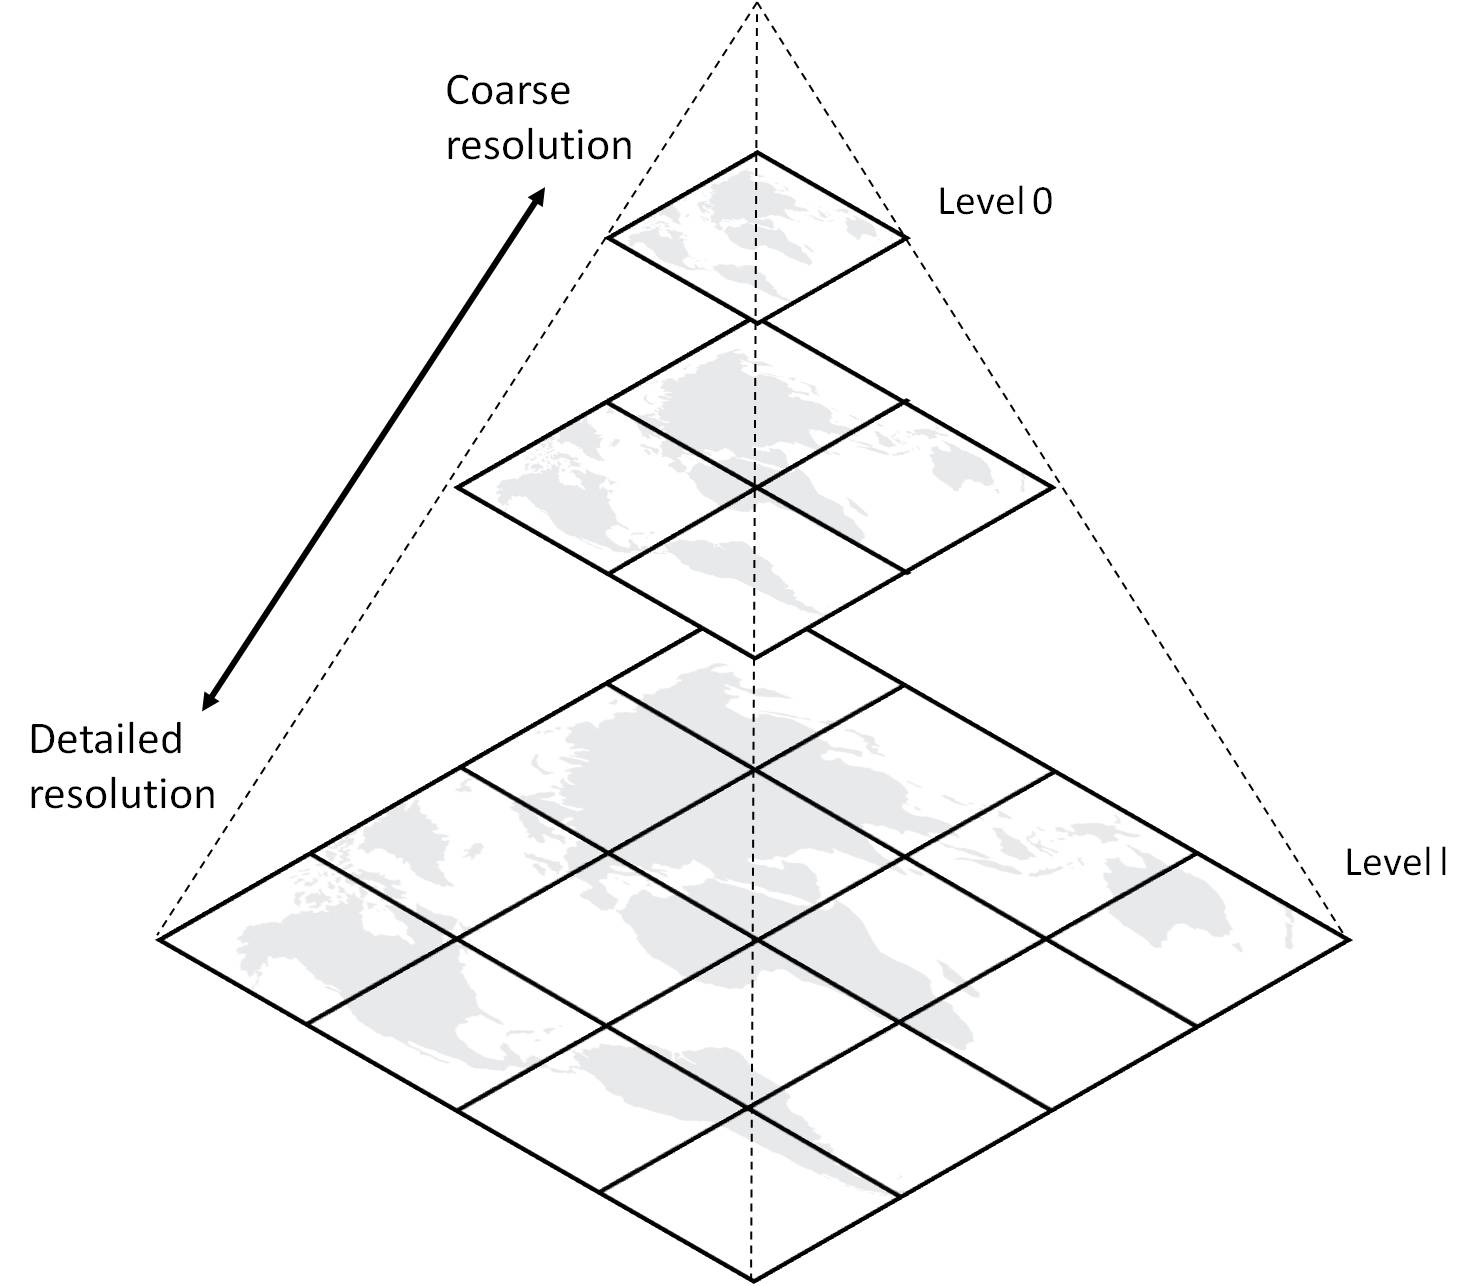
\includegraphics[width=0.4\textwidth]{figures/TilePyramid.jpg}
    \caption{Tile pyramid representation \cite{garcia12}}
    \label{fig:tile_pyramid}
\end{figure}

In the context of tile maps, two formats are primary used for serving tiles. The widely used raster tile maps and the newer vector tile maps \cite{netek_performance_2020}. Raster tile maps store for each tile on each level an image of fixed sized (most commonly 256x256 pixels) \cite{garcia12}. The client sends a request to the server requesting an image tile at the current layer (zoom factor) $z$ and the $x$ and $y$ location of the image. Each image tile in one layer is identified by a coordinate tuple $(x, y)$ beginning with $(0,0)$ in the top left corner. The Open Geospatial Consortium has standardized on how to serve image tile maps \cite{noauthor_opengis_nodate}. The biggest disadvantage of raster tile maps is that updates to the map data always requires generating new tiles for the affected parts of the map \cite{netek_performance_2020}. This case is not present when looking at vector tile maps. The tiles are not images, but only contain vector data of the geometric elements point, line and polygon. Vector tile maps support fractional zoom levels (e.g. $z=8.5$) which is not supported by raster tile maps. The information of a vector tile is mostly stored in the GeoJSON, TopoJSON or Mapbox Vector Tile format (mvt) \cite{netek_performance_2020}. Mapbox is a commercial map service which also tries to standardize different map rendering techniques and API schemes. Their vector tile format uses the Google Protobufs format (PBF), which allows for serialization of structured data \cite{noauthor_vector_nodate}. OpenStreetMap also uses this format to serve their map data as an alternative to XML, because it results in significantly smaller file sizes \cite{noauthor_pbf_nodate}. Vector tiles do not contain any style information. Styles have to be defined by the client in a corresponding stylesheet. A stylesheet contains a reference to the data in the vector tiles and rules on how to render this specific data (e.g. how a house should be rendered) \cite{netek_performance_2020}. There are multiple standards and specification in existing \cite{noauthor_cartocss_nodate}\cite{noauthor_cartocss_nodate}. Mapbox created the Mapbox Style specification, which is compatible with the \textit{mvt} format. A stylesheet is defined inside a JSON-object \cite{noauthor_style_nodate}.

Raster tile maps do not offer the flexibility that the rendering service needs. Events from the Changeset-Watcher would result in a renrender of all affected tiles. Furthermore, styles can not be dynamically defined by the user. Thus, the implemented rendering service uses vector tile maps. 

PostGIS is an extension for the object-relational database PostgreSQL, which adds support for spatial data and queries \cite{noauthor_postgis_nodate}. Since version 2.4.0 PostGIS offers two functions \texttt{ST\_AsMVTGeom} and \texttt{ST\_AsMVT}. The prior transforms geometry columns into the coordinate space of a Mapbox Vector Tile. To define which geometry should be included in the tile, a bounding box must be passed to the function \cite{noauthor_st_asmvtgeom_nodate}. The latter function allows aggregation of multiple rows and returns a Mapbox vector tile in binary format \cite{noauthor_st_asmvt_nodate}. As the functions can be used in SQL-queries, updates made to the used geometry columns are reflected in the vector tile, when the query is executed again.

There are numerous Open Source solution in existing which combine the use of a PostGIS database for storing OSM data and the serving of vector tiles via HTTP-requests \cite{noauthor_awesome-vector-tiles_2022}. The two main solutions, we were considering, were \textit{Martin} \cite{noauthor_martin_2022} and \textit{Tegola} \cite{noauthor_tegola_2022}. Martin offers the functionality to autodetect existing spatial tables and automatically offers HTTP-endpoints for each table. Those endpoints can be queried to receive different information about the table, including serving Mapbox Vector Tiles \cite{noauthor_martin_2022}. Tegola does not offer this feature. It needs a TOML-configuration file, in which the PostGIS provider and tables need to be defined by hand \cite{noauthor_tegola_2022}. Additionally, you have to define which maps should be exposed on an HTTP-endpoint. While testing both server with the same PostGIS database, we did not notice that one server was more performant serving vector tiles than the other. We finally selected Tegola as our vector tile server as it is more customizable than Martin. Especially when defining which data should be included in the vector tiles.

Listing \ref{listing:tegola_config} shows a minimal configuration file for Tegola. Multiple different providers with different types can be defined. Additionally, multiple provider layers can be specified. Each layer corresponds to a table in the database defined by the key \texttt{tablename}. The value of the key \texttt{sql} defines which data should be included in the vector tile. The function \texttt{ST\_AsMVTGeom(geometry,!BBOX!)} returns the vector tile. The \texttt{!BBOX!} statement is automatically replaced by Tegola by the bounding box the client requested in the HTTP-request. Additional columns can also be selected, which make it possible for the client to render different attributes, e.g. the name of a street. To make the vector tiles accessible to the user, a map layer needs to be defined. The important keys are \texttt{min\_zoom} and \texttt{max\_zoom}. Those define on which zoom level the data should be included in the vector tile. This makes it possible to query different tables for different zoom levels. 
For example, on a very low zoom level, where Germany fits into one vector tile, it is not performant to render all forest at their maximum geometric resolution. Therefore, for different zoom levels, different tables or columns are used to return different geometric resolution.

\begin{listing}[h]
    \inputminted[tabsize=2, fontsize=\footnotesize]{python}{listings/tegola.toml}
    \caption{Example Tegola configuration for a provider layer and a corresponding map}
    \label{listing:tegola_config}
\end{listing}

As rendering should generally render all information included in the OSM data, the rendering service listens to the \textit{all}-subject of the Changeset-Watcher. The data from this subject is in the OsmChange format and compressed. This format of the data is needed for the update routine of the PostGIS database. As a PostGIS database is used for storing the rendering data, a solution for incrementally updating the database is needed. The two main solutions we were looking at were \textit{Imposm} \cite{noauthor_imposm_2022} and \textit{osm2pgsql} \cite{noauthor_osm2pgsql_2022}. Where the latter is the more common used tool. But we found Imposm more easily to develop with. Especially because the database schema can be defined in a JSON- or YAML-file, while osm2pgsql needs custom scripts written in Lua to define the schema of a table \cite{noauthor_imposm_2022}\cite{noauthor_osm2pgsql_nodate}. In the specific JSON-file a mapping is defined of which OSM elements and tags should be included in the database. Imposm then creates a corresponding database schema. Imposm offers the functionality to apply OSMchange files to the database. Due to Tegola's usage of SQL-queries for the generation of vector tiles, the applied changes are reflected in the vector tile on the client's next request for the affected tiles. As figure \ref{fig:renderer_squence} shows, updating and querying of the PostGIS-database happens in parallel. A restart of the Tegola server is therefore not needed. With the downside that eventual consistency can appear, if the client does not request the updated tiles. But this only happens on rare occasions because a client normally often zooms and pans in its viewer and therefore often requests the same (updated) tiles. 
\begin{figure}[h]
    \centering
    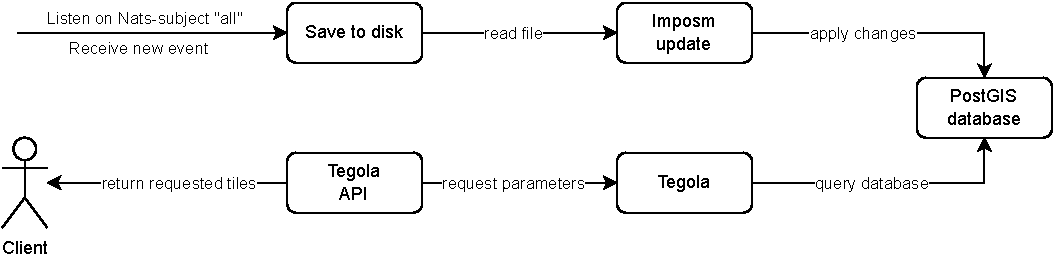
\includegraphics[width=0.48\textwidth]{figures/renderer.pdf}
    \caption{Updating and querying of the rendering service}
    \label{fig:renderer_squence}
\end{figure}

\subsection{Routing}
\label{subsec:Routing}
The last exemplary service we implemented is a routing service. Routing in our context means, finding the fastest path from point A to point B on a street network. Because streets in OSM are stored as simple way-elements with corresponding tags, they can not be used for efficient routing. To run efficient path finding algorithms, the street data needs to be converted into a graph structure. Numerous routing engines already exists, which can convert OSM data in their used routing format and offer fast routing capabilities. The ones we were looking at more thoroughly, were \textit{Graphhopper} \cite{noauthor_graphhopper_2022}, \textit{Valhalla} \cite{noauthor_valhallavalhalla_2022}, \textit{Open Source Routing Machine} \cite{luxen-vetter-2011}. 
Our goal was that update events should also be reflected instantly in the routing service. But none of the named engines support incremental updates. There are GitHub-Issues and discussion for such a feature, but no engine implemented it until this day \cite{noauthor_update_2021}\cite{noauthor_can_nodate}\cite{noauthor_incremental_nodate}. Therefore, we experimented with a solution where incremental updates would be possible. Based on a blog-post \cite{rodrigo_imposm2pgrouting_2020} we tried implementing a routing engine based on \textit{pgRouting} \cite{noauthor_pgrouting_nodate} and database triggers for routing database updates. The solution seemed promising, but street updates were not always correctly reflected in the routing network. Furthermore, configuring pgRouting was a tedious process, as everything needs to be expressed in SQL-queries and the rules for edge cost need to be defined by the user. Due to the limited project time, we decided to stop this experiment and use one of the existing routing engines. Evaluating the different routing engines, we found the Open Source Routing Machine (OSRM) easiest to handle with and connect to our events. To generate the routing structured, an OSM file is needed. OSRM then preprocesses and converts the contained streets into their routing structure. 
As no updates to the OSRM routing structure are possible, we have to keep a local OSM-file up-to-date. This local map only contains information about streets, as no other data is needed by OSRM to generate the routing structure. The configuration file for the CSW, already shown in \ref{list:routing-configuration}, hence filters for the \texttt{highway}-tag. As figure \ref{fig:routing_bpmn} shows, the received event is saved to the local file system and afterwards applied to the local map. For updating, the command line tool Osmium \cite{noauthor_osmium_2022} is used. It makes it possible to apply OsmChange files to an OSM file. To update the OSRM routing structure, a Cronjob runs the necessary steps every five minutes (see figure \ref{fig:routing_bpmn}).
\begin{figure}[h]
    \centering
    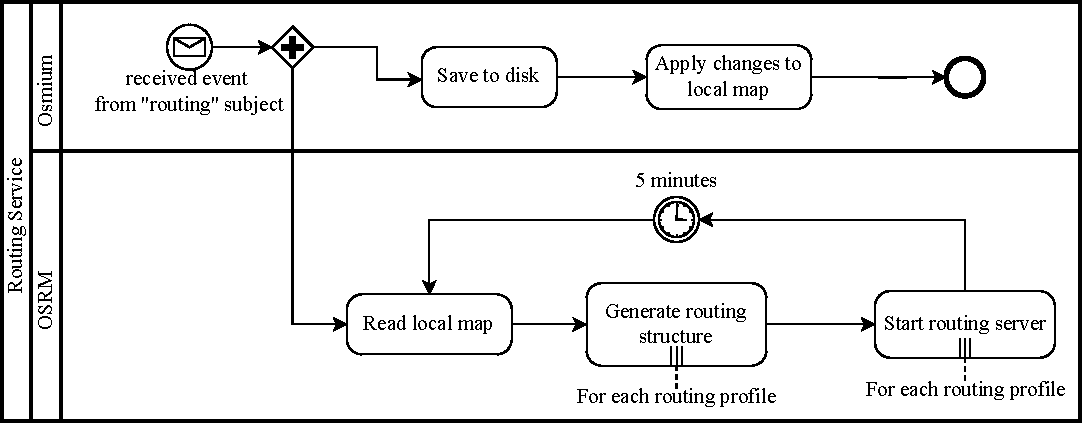
\includegraphics[width=0.48\textwidth]{figures/routing.pdf}
    \caption{Process of routing service on a received event}
    \label{fig:routing_bpmn}
\end{figure}
OSRM offers the functionality to implement different routing profiles. Car, bicycle and foot profiles are already predefined. Those profiles take into account that a route for a pedestrian or bicycle should not contain any street types, that are not suitable for them, e.g. highways. To offer routing for different profiles, a routing structure needs to be generated for each profile. Each profile runs on its own OSRM server instance, resulting in three different REST endpoints. The routing structure for each profile is saved in a corresponding OSRM file. OSRM hence does not use any database or other additional software, but stores all its needed data in files on the file system. The duration for generating the files for each profile increases significantly with increasing size of the street network in the local map. As high availability is important, we can not shut down the server instances until the generation is finished. Therefore, the new routing structure is written to a temporary folder. Thus, the routing service is only turned off when the temporary folders need to be swapped with the production folders. Resulting in a relative constant downtime of a few seconds compared to multiple minutes or hours, if the local map contains a lot of streets.
Each profile uses the same Rest-API offered by the OSRM server instance. Our routing services then expose those endpoints on different ports, so each profile can be queried independently.

\subsection{Frontend}
\label{subsec:Frontend}
To make the three services easily visible and usable for users, we created a simple web user interface. It is based on VueJs \cite{noauthor_vuejs_nodate}, a well known JavaScript Framework. It makes developing Single Page Application (SPA) easy and fast. For displaying the vector tiles, we use the Open Source fork of Mapbox GL JS named MapLibre GL \cite{noauthor_maplibre_2022}, which is a library for creating interactive vector maps in the browser. As already mentioned in section \ref{subsec:Rendering}, vector tiles do not contain any style information. Hence, we created our own stylesheet compatible with the Mapbox Style Specification. Instead of defining everything in a JSON-object we stored our styles in JavaScript Objects, which make it easy to enable and disable certain parts of the map. As we are using TypeScript, we also have the benefit of type-safety while defining our styles, as the specification offer corresponding TypeScript types. Listing \ref{list:style_example} shows an exemplary style definition for buildings. The mapping from the data in the vector tiles to the style definition is defined by the properties \texttt{source} and \texttt{source-layer}. As the map library allows loading tiles from multiple sources, the general source has to be referenced by its name. The \texttt{source-layer} corresponds to the name defined in the Tegola map-layer shown in listing \ref{listing:tegola_config}.
\begin{listing}
    \inputminted{ts}{listings/style_building.ts}
    \caption{JavaScript Object defining the building styles}
    \label{list:style_example}
\end{listing}
All style definitions combined creates a map, which can be seen in figure \ref{fig:frontend_search}. Additionally, the connection to the search API is shown. In the top left corner the user can type search queries into the input field and for every letter typed the search API returns the best fitting results. Each result is visualized as a separate card and a marker is added for its geographic position on the map. The map also adjusts itself in a way that all markers are visible for the user. Clicking on one of the search results focuses it and the map zooms to it (as shown in figure \ref{fig:frontend_search}). In the bottom left corner, the current amount of search items in the search database is visualized. Every 30 seconds, it will check via polling for a new amount. 
\begin{figure*}[h]
    \centering
    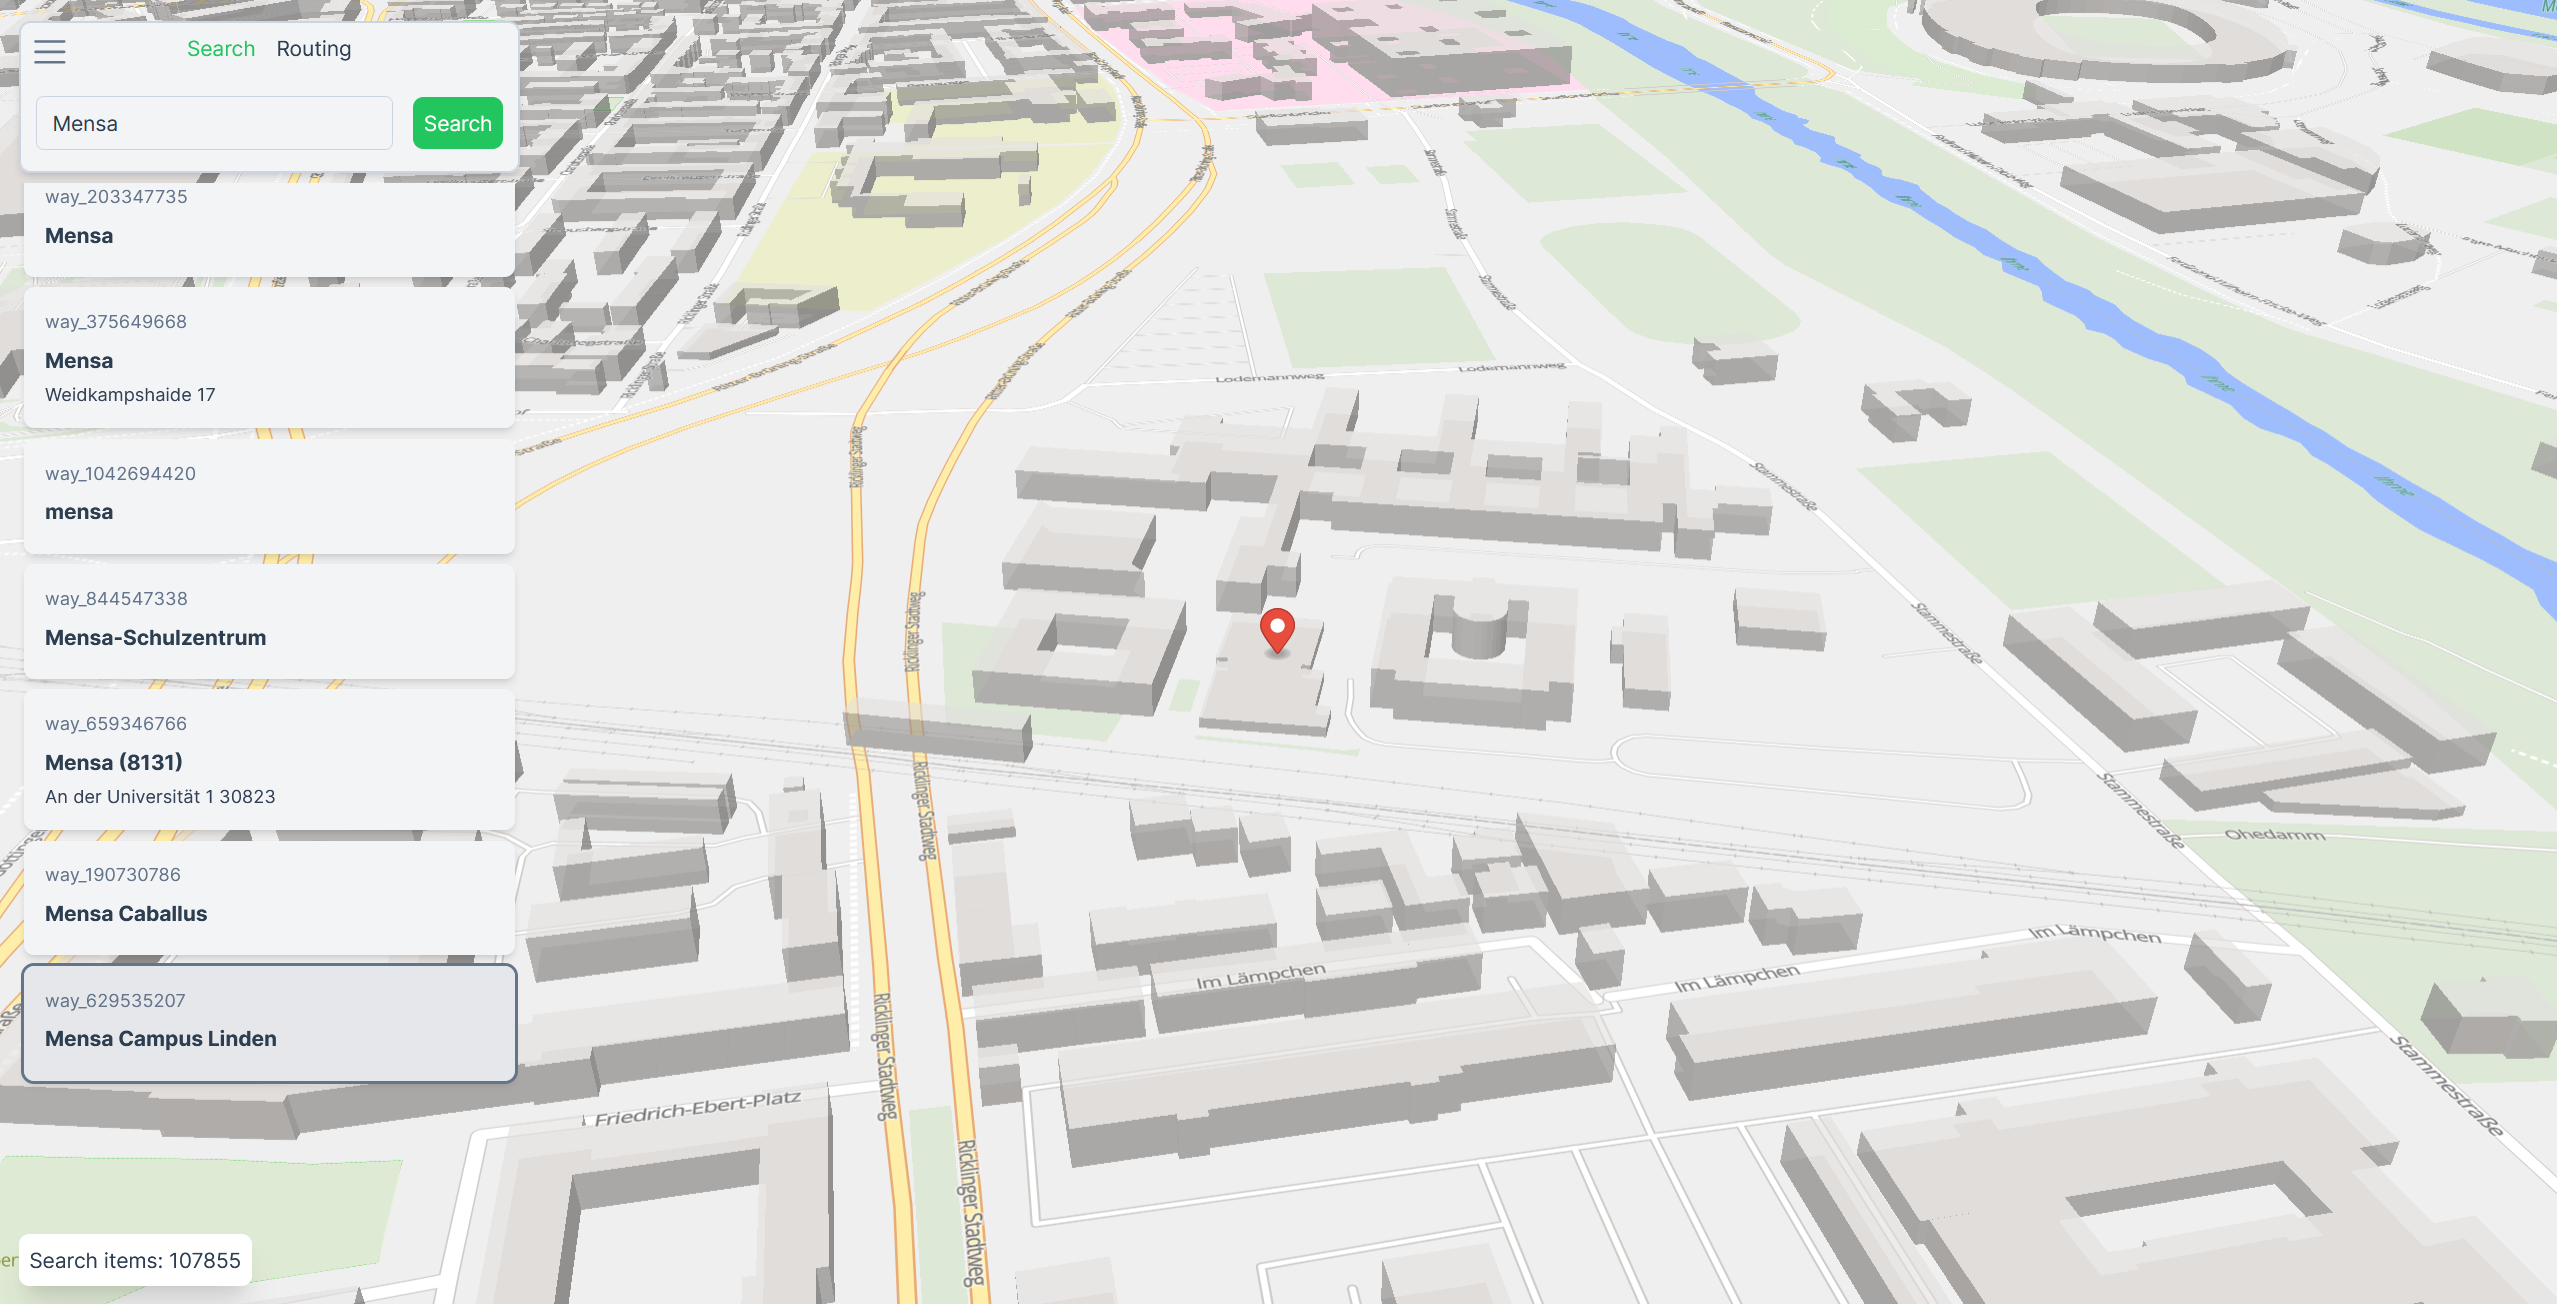
\includegraphics[width=\textwidth]{figures/Mensa.png}
    \caption{Web user interface with search results with imported data from Hanover, Germany}
    \label{fig:frontend_search}
\end{figure*}

To interact with the routing service, a separate routing tab is offered. The user can search for a start and end point. For finding the corresponding geographic positions, the same search representation as described is used both for the start and end point. The user can also select the profile it wants a route for. This is visualized in figure \ref{fig:frotend_routing_car} and figure \ref{fig:frotend_routing_foot}. We calculated a route from the cafeteria of the Hochschule Hannover to the caferia of the Leibniz University Hannover. The geometry information of the calculated routes is returned by the routing service and visualized with a polyline on the map. As can be seen, the calculated route differs depending on the selected profile. This is also noticeable in the card which is located under the destination card, where the estimated duration and distance is displayed. Additionally, the amount of navigational steps e.g. Turn left in 300 meters on street x, is shown. Due to time constraints, we could not visualize all steps, to instruct the user how exactly he gets from his start point to his wished destination.

As already mentioned in the previous sections, updates made to any service are always instantly reflected in the web user interface after the processing of them is done. Mostly noticeable at the different search item count visible in the figures \ref{fig:frotend_routing_car} and \ref{fig:frotend_routing_foot}.

\begin{figure}[H]
    \centering
    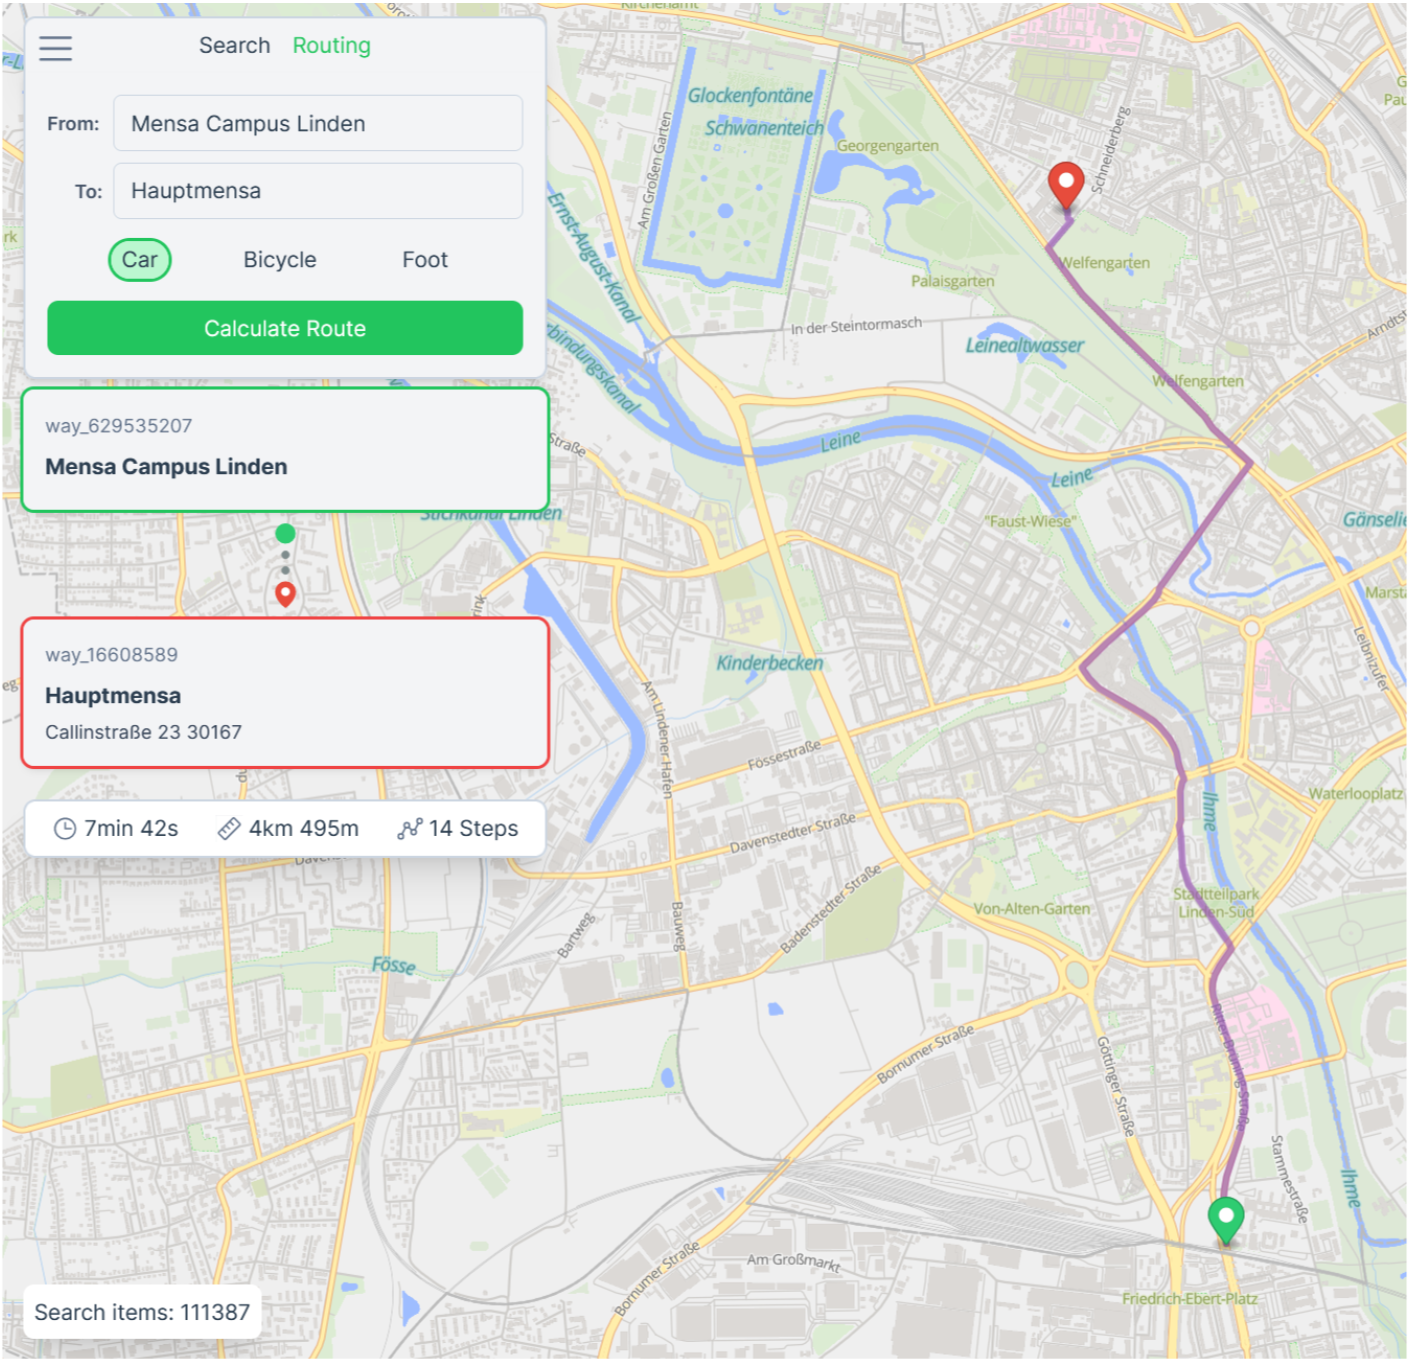
\includegraphics[width=0.35\textwidth]{figures/routing-1.png}
    \caption{Web user interface for routing with car profile selected}
    \label{fig:frotend_routing_car}
\end{figure}

\begin{figure}[H]
    \centering
    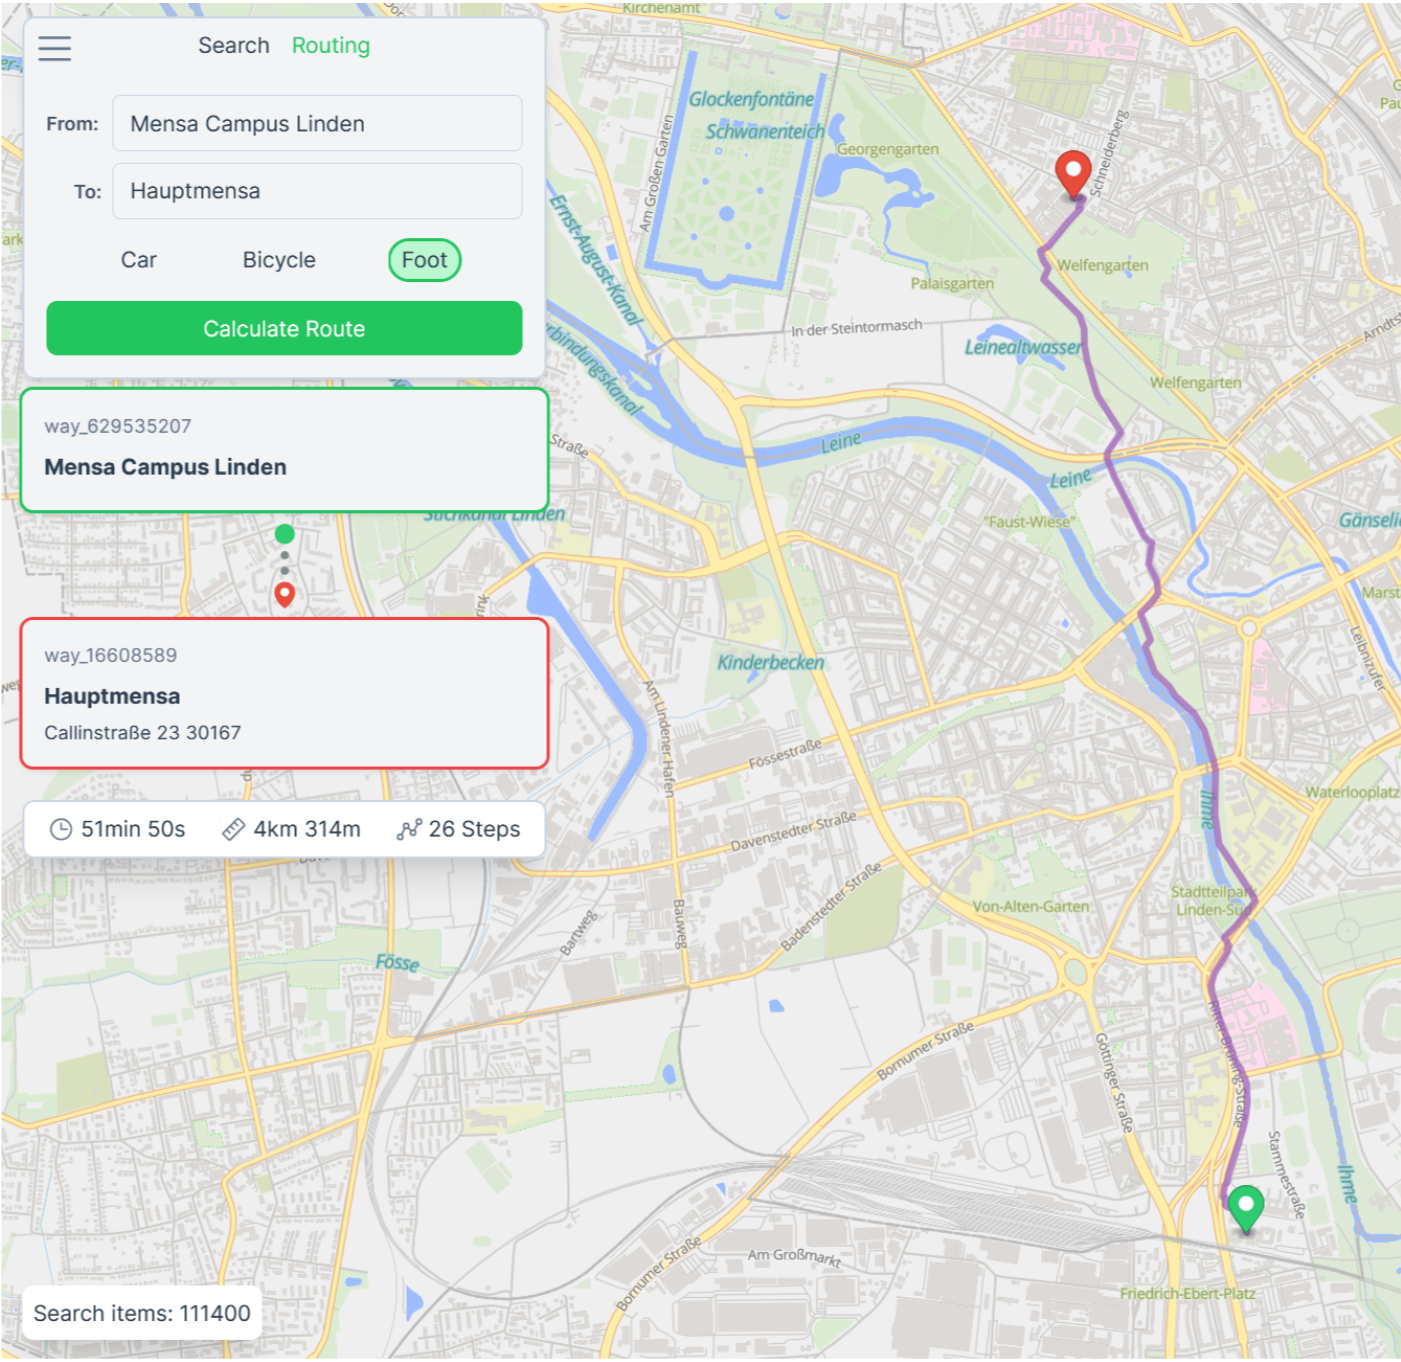
\includegraphics[width=0.35\textwidth]{figures/routing-2.png}
    \caption{Web user interface for routing with foot profile selected}
    \label{fig:frotend_routing_foot}
\end{figure}

\section{Results}
\label{sec:Results}
As already mentioned in section \ref{sec:preprocessing} our current implementation uses the minutely published changesets provided by OSM. This results in the requirement that our Changeset-Watcher must be capable of processing every new changeset in under one minute. So every event is published to Nats before a new changeset is available. To verify this requirement, we deployed our pipeline on a server for one week. As all services are running in separate Docker Container the deployment with Docker Compose was fairly easy, as the Nats events are the only communication between the Changeset-Watcher and the different services. The server contains four dedicated cores and 16 GB of memory. Our prototype was not the only Docker Container running on this server. Hence, the gathered results could be affected by the other containers using server resources.

In general, the Changeset-Watcher processed 9\,951 changesets. All changesets combined result in a total of  49\,780\,431 OSM elements of type node, way or relation. There were also 9\,951 events published to each service. To find out how effective the filtering for each service is, it was counted how many elements are contained in one event. As the \textit{all}-subject, used by the renderer, does not have any filtering, the number of published elements is equal to the number of elements contained in the received changesets. The \textit{routing}-subject received 15\,987\,375 elements. Hence, roughly 67.88\% of elements were not published on this subject. The \textit{search}-subject has even greater filter minimization, as only 779\,513 elements were received. That results in 98.43\% of not published elements. That shows that the filtering in general is very useful and reduces the load on the event bus and on the services, as they have to process significantly fewer elements.

The second metric is the time needed for the Changeset-Watcher to process a received changeset. This duration can be divided into two sub-metrics. The time needed for executing the specific filter configuration for one subject and secondly reloading all missing nodes from the overpass-API. Figure \ref{fig:time_comparison_diagram} shows for each subject the time needed for executing their specific filter configuration in relation to the number of incoming elements.
The size of one data point is in relation to the number of elements that were published to the subject. For better visibility, clear outliers, caused by server lags, were removed from the dataset. Each subject shows a high variety in processing time of different size. The \textit{all}-subject suggests a linear growth factor with increasing element amount. This is obvious, as the filter configuration only compresses the elements. The \textit{search} and \textit{routing}-subject on average show processing durations of several hundred milliseconds. As only a low percentage of elements pass the search filter configuration, the duration is normally very low. But as the configuration also reduces the elements to searchpoints, the calculation effort is generally higher. One changeset included 37\,252 elements that fulfilled the search filter configuration. The Changeset-Watcher needed 107.862 seconds to process those. This was the only occurrence of a changeset where the processing needed longer than a minute. This is also reflected in the mean and median of all three configurations. The \textit{all} configuration showed a mean of 68.7165 milliseconds and a median of 57 milliseconds. Followed by the \textit{routing} configuration with a mean of 31.8180 milliseconds and a median of 25 milliseconds. As expected, the \textit{search} configuration was the fastest, with a mean duration of 19.8928 milliseconds and a median of 1 milliseconds.

Missing nodes in changeset are fetched from the overpass-API. This brings the risk, that our system is dependent on the response time of the provided enpoint for nodes reloading. Besides the general problem, that the Changeset-Worker will not work, if the overpass-API is offline. This case did not occur in the week of testing. Diagram \ref{fig:reloading_nodes_statistic} shows that the reloading always needed less than one minute. Even the one changeset that resulted in reloading nearly 160\,000 thousands nodes needed just below 30 seconds. On average the node reloading took 3.834 seconds.
\begin{figure}[h]
    \centering
    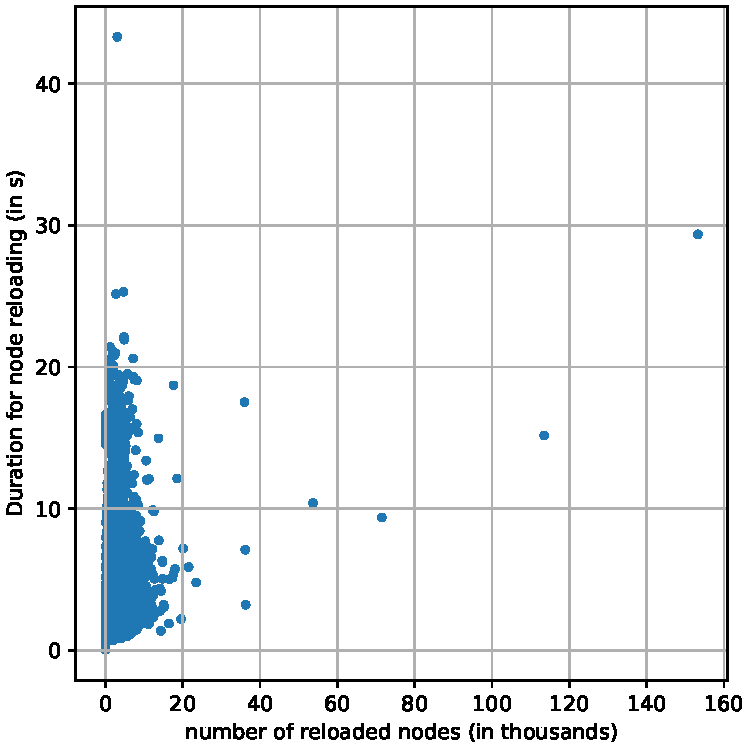
\includegraphics[width=\textwidth/2-2cm]{figures/reloaded_nodes_statistic.pdf}
    \caption{Duration for reloading missing nodes from the overpass-API}
    \label{fig:reloading_nodes_statistic}
\end{figure}

Additionally to the performance of the Changeset-Watcher, the duration for each service to update its data structure was documented. Figure \ref{fig:renderer_diagram} shows the duration needed by Imposm to update the PostGIS database over increasing time. Nearly every update is below the border of $60$ seconds, where a new event could occur. Some data points clearly deviate from the norm. Those points are highly caused by server lags, because events of similar size took significantly less time. On the right diagram, a slow, but noticeable overall increase in update time is visible, due to the increasing size of the database. But updates are still under $4$ seconds. The week of updates resulted in a median of 887 milliseconds.

Looking at the routing service, we see a similar result. Updates with Osmium are generally slower compared to Imposm. The same server caused outliers are noticeable (see left diagram \ref{fig:routing_diagram}). Overtime the general update duration increases significantly. At the end, updates were between 7 and 10 seconds. The median over the seven days was 4.28 seconds. Another linear increase can be observed in the file size of the local map. This was expected, as the map is created from an empty world. At the end the file had a size of 140 MB (see middle diagram \ref{fig:routing_diagram}). As mentioned in section \ref{subsec:Routing}, for each routing profile, a routing structure must be generated. As the street networks grows, it was expected that the generation will need longer. The right diagram in figure \ref{fig:routing_diagram} proves this. It shows the generation duration for all routing profiles combined. Many spikes are visible, which is again due to limited server resources, as the generation process is very CPU and memory intensive. In general, a linear increase in generation time can be recognized. That the generation duration quickly jumps above one minute was expected and is compensated by the use of temporary directories described in section \ref{subsec:Routing}.

The search service showed the lowest update durations. The median resulted in $35.45$ milliseconds. Those low update durations are mostly due to the fact, that the received events on average contain 78 elements (compared to the 1606 elements in the routing service). When the search service received events with hundreds or thousands of elements, there were also update durations of multiple seconds noticeable. Generally, there was no linear increase in the update duration with increasing index size observable, like with the other services. 

\section{Discussion}
\label{sec:Discussion}
The implementation showed that the CQRS pattern can be easily applied to spatial data. The Changeset-Watcher (CSW) makes it possible that services of the read model only receive the data that they need for their use case. The collected metrics showed that filtering the data is very useful. The CSW allows that services do not need to do any filtering of the data. Therefore, reducing the load on the services.
Scalability of services can also be easily applied. Each service of the read model can be scaled independently. The routing service for example could be deployed on three different servers. Each server running an OSRM routing instance for one of the three routing profiles. As the CSW itself is implemented with parallelization in mind, each filter configuration is processed in its own thread.   

The collected metrics showed, that the CSW and the services are capable of processing a changeset before a new one arrives. Disadvantageous is the current consistency and fault tolerance. As observed, it can happen that a changeset is big enough, that the CSW needs more than a minute to process it. If the next changeset is very small and therefore processed very fast, the event order gets mixed up, as they are processed in parallel. This can lead into an inconsistent state or even cause errors at the connected services. Therefore, the CSW should be extended with a check procedure for each filtering configuration, so the events get published in the right order.

Another disadvantage with the current implementation is that already processed events are not saved in any form. If an already connected services fails to receive events for a period of time, it has no chance of recovering the missing state changes on the write model, resulting in inconsistencies. Moreover, if a new service connects, it can not fetch all previous events and has to start from the newest event published by the CSW. To compensate for this, each event published could contain some sort of sequence number, so each service can determine if it has missed events. The CSW then has to offer the functionality to republish events for the received range of missing sequence numbers. Either storing every event for each sequence number or reproducing it from the \textit{planet.osm} changesets. For single lost events, the acknowledgement feature of NATS could be used to resend events to the subject \cite{noauthor_acknowledgements_nodate}.

Currently all nodes missing in a changeset will be reloaded from the overpass-API. To be less dependent on this external service, the CSW could store all already reloaded nodes internally. A key-value store with the node ID as key could be helpful here. Then only those nodes not in the store must be reloaded, which could also improve overall processing time of a changeset. 

The disadvantages just mentioned do not in any way exclude the application of the CQRS pattern to spatial data. It is possible to reduce or even eliminate these disadvantages by extending the implementation with the presented concepts. Moreover, the effect of filtering can be significantly enhanced by extending the CSW. Besides filtering of elements that have certain tags, filtering of geographical regions is also possible. Services could thus subscribe to regions they are interested in.

\printbibliography

\bibliographystyle{IEEEtran}
\bibliography{bibi.bib}

\newpage\phantom{x}

 \appendices
 
   \section{Metrics}
  \label{appendix:graphics}
  
 \begin{figure}[!ht]
    \centering
    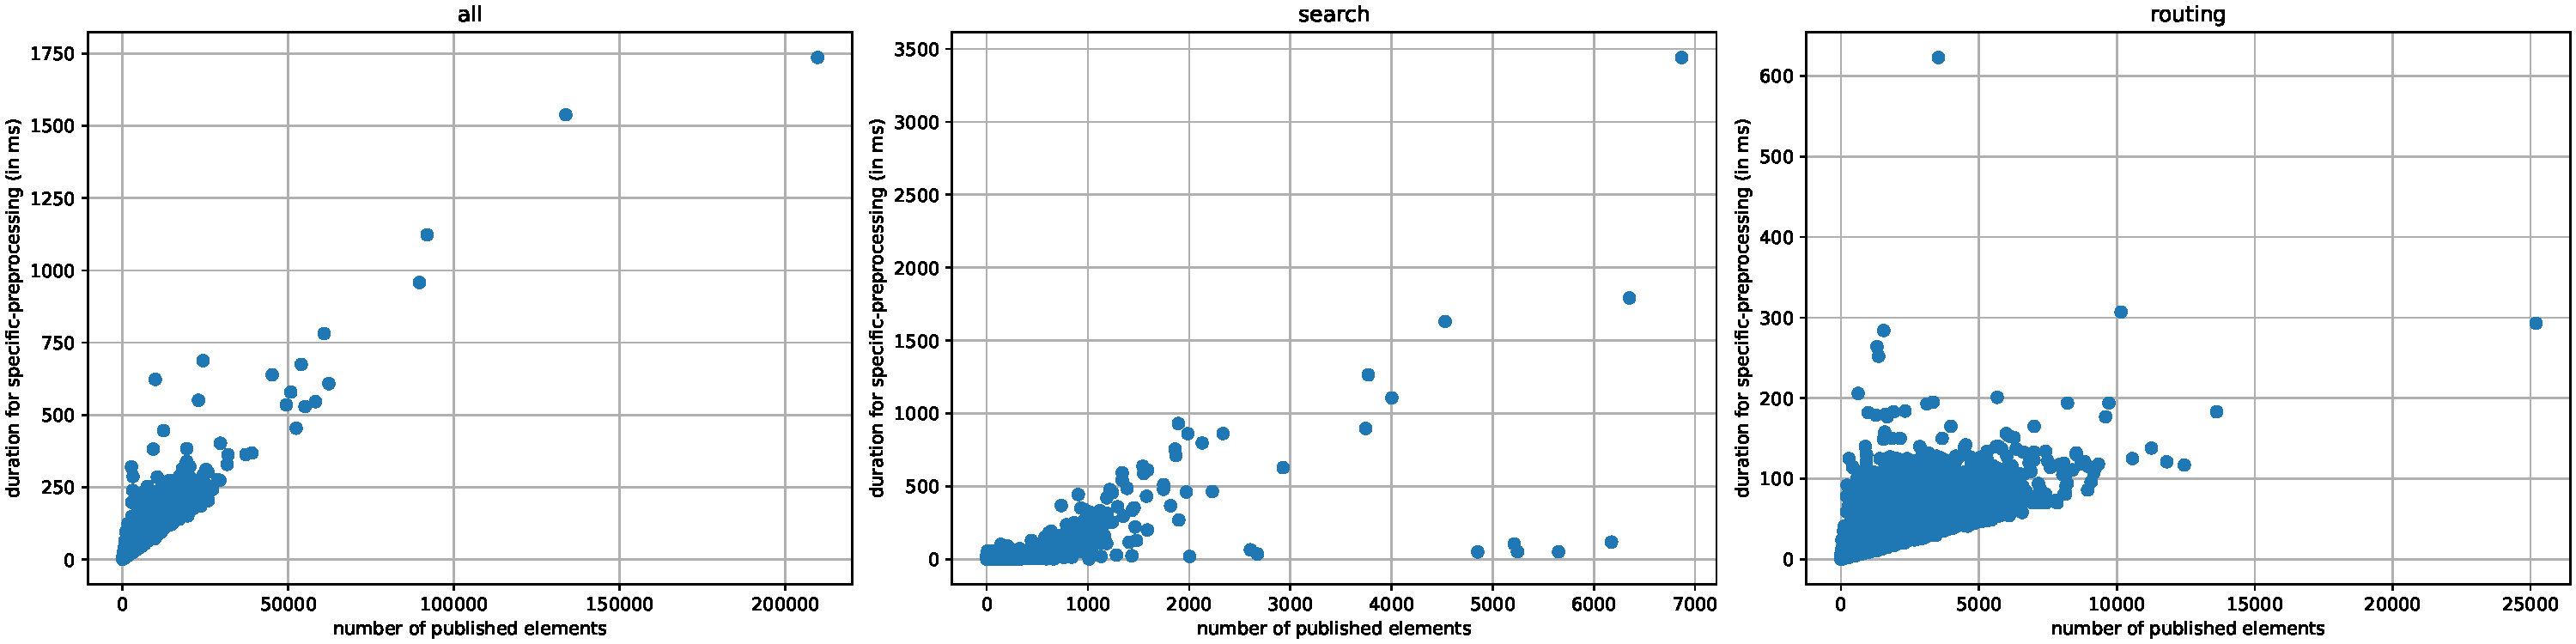
\includegraphics[width=\textwidth]{figures/subject_filtering_comparison.pdf}
    \parbox{\textwidth}{\caption{Time needed for each filter configuration to filter and process the incoming events}}
    \label{fig:time_comparison_diagram}
\end{figure}
 
  \begin{figure}[!ht]
    \centering
    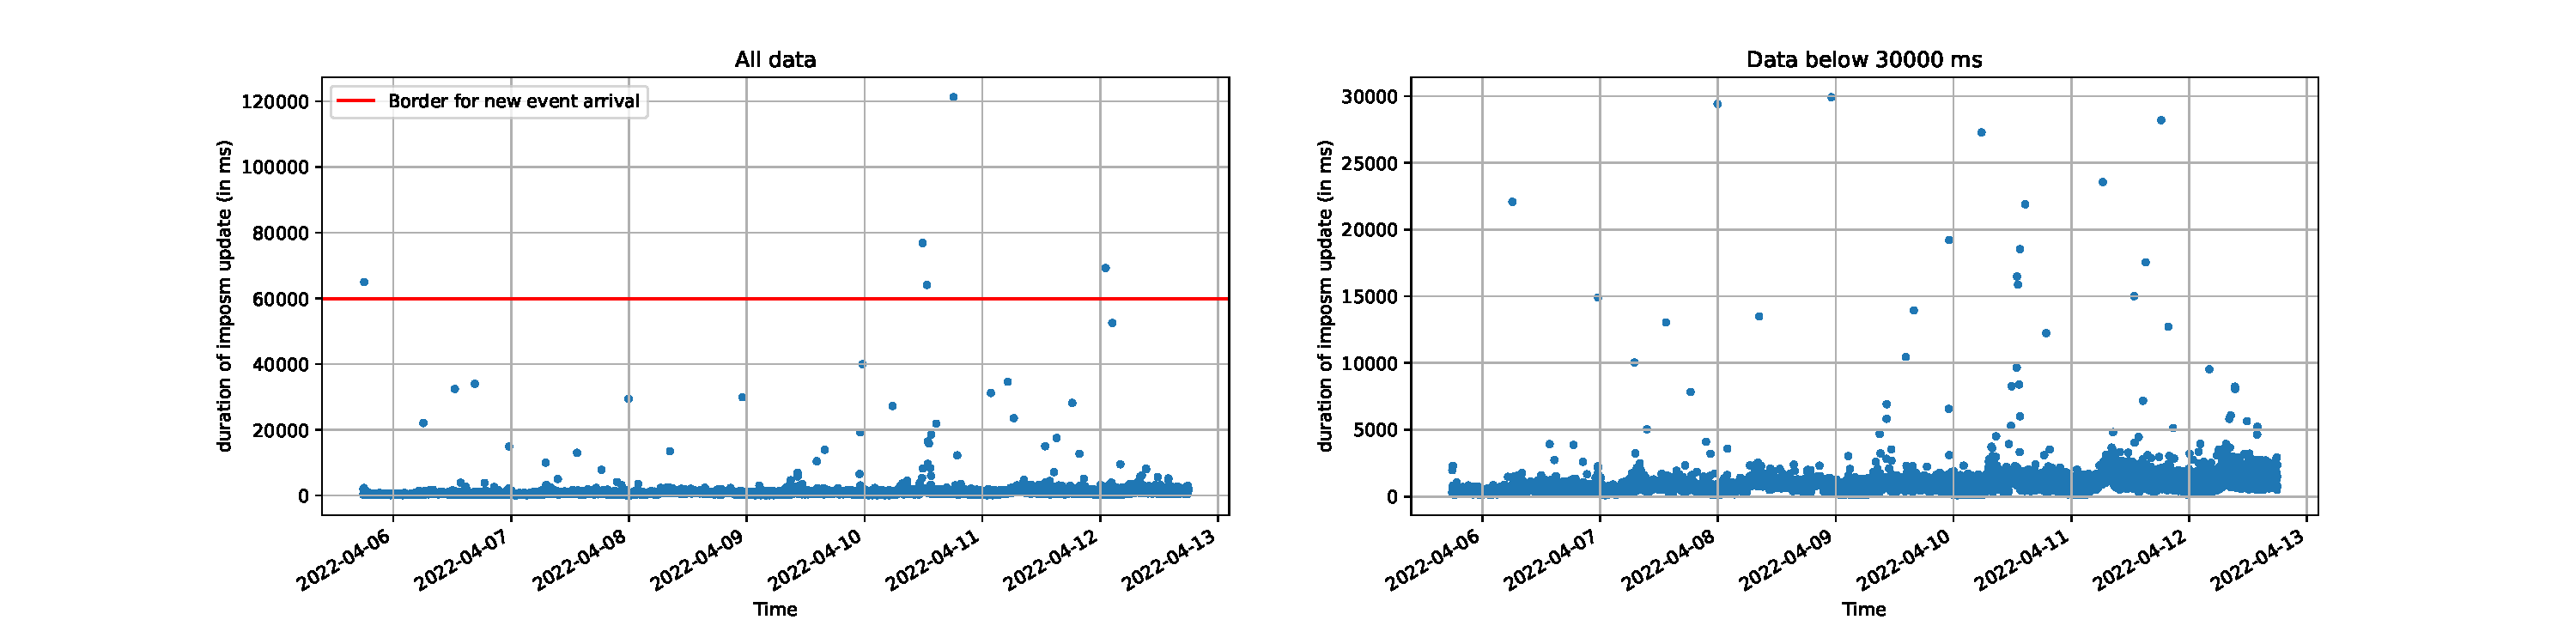
\includegraphics[width=\textwidth]{figures/renderer_statistic.pdf}
    \parbox{\textwidth}{\caption{Duration of all Imposm updates (left) and updates below 30 seconds (right)}}
    \label{fig:renderer_diagram}
\end{figure}

\begin{figure}[!ht]
    \centering
    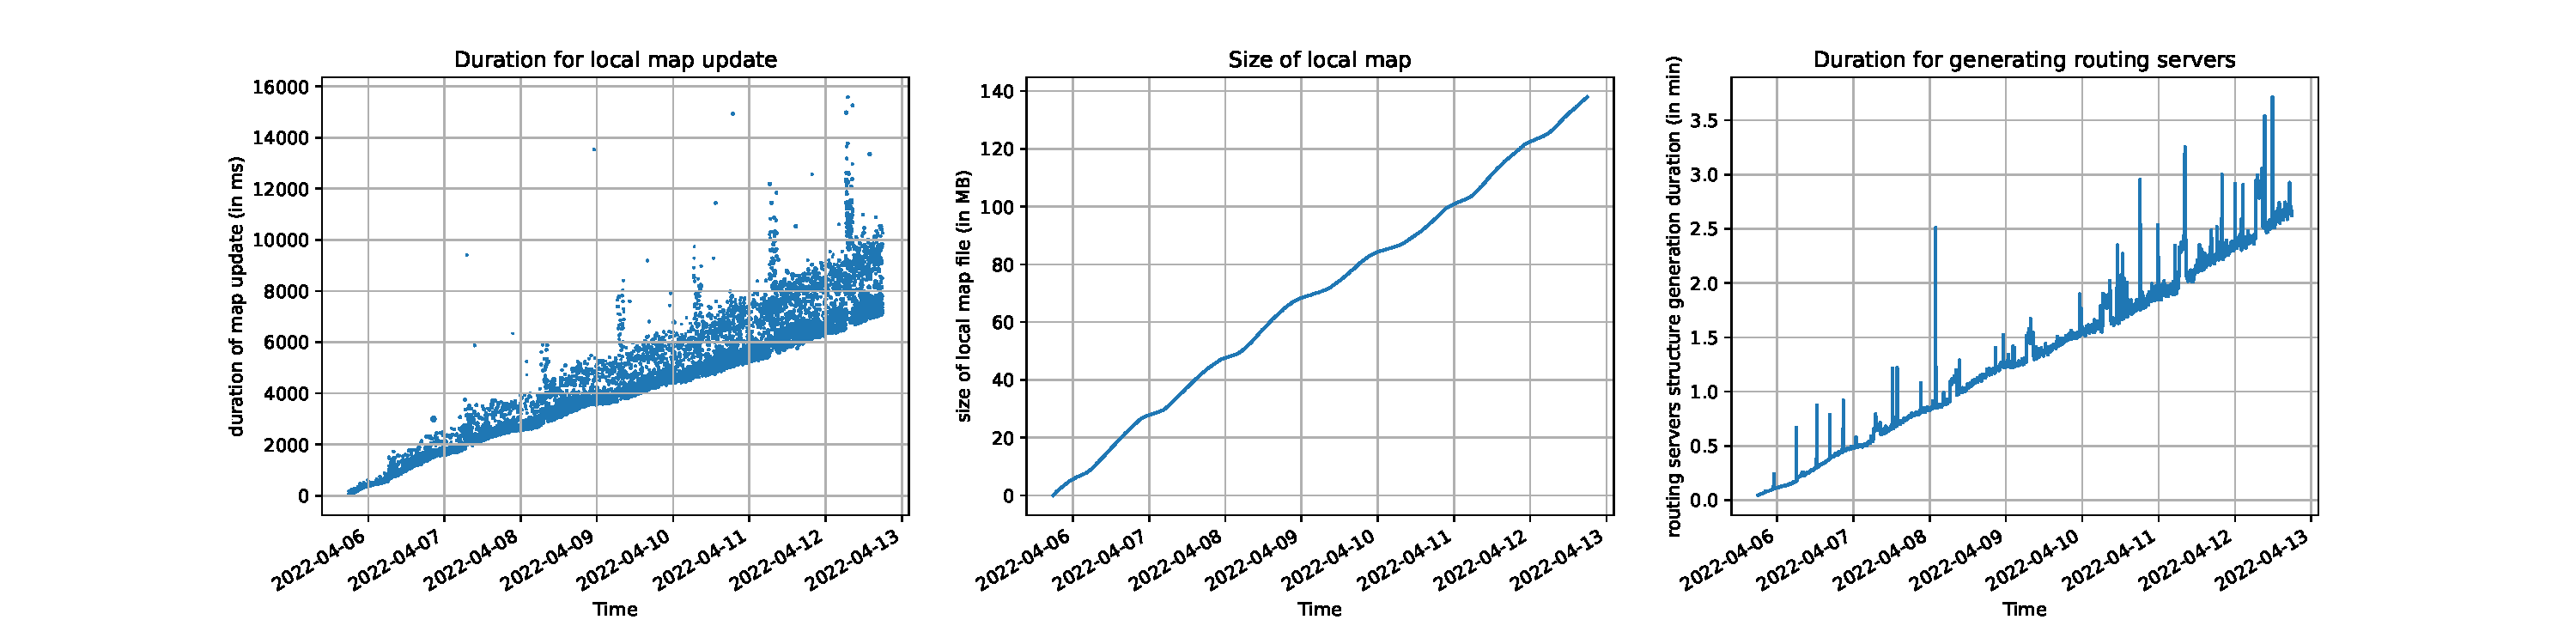
\includegraphics[width=\textwidth]{figures/routing_statistic.pdf}
    \parbox{\textwidth}{\caption{Duration of Osmium map update visualized on left. The size of one data point relates to the event size. Middle diagram visualize the size of the local map file over time. The right diagram visualizes the duration for generating the three routing servers. }}
    \label{fig:routing_diagram}
\end{figure}
\end{document}
